\section{Real-time implementation}
\label{sec:rt}

The application consists of a
static GTFS~schedule and network data component,
and a \rt modeling and prediction component.
We chose \verb+Rcpp+ to develop the program,
providing access to other R packages for data manipulation 
(notably \verb+RSQLite+ and \verb+dplyr+),
as well as the speed and memory management capabilities of \verb|C++|. 
The following has been implemented in the R package
\verb+transitr+, available on Github (\url{https://github.com/tmelliott/transitr}).
In this section, we discuss the features of the \rt component.

The general structure of the \rt component is shown below,
with the bold steps being those discussed in this paper.
\begin{enumerate}
\item Load GTFS data from database
\item Indefinitely repeat when new data recieved \ldots
\begin{enumerate}
    \item Update or create new vehicle objects from new data
    \item \textbf{Run particle filter on each vehicle to update state}
    \item \textbf{Update state of any roads for which vehicles 
        have completed travel}
    \item Generate ETAs for vehicles uing combination of particle filter and network state
    \item Write ETAs to extended Google Protobuf binary file for distribution
\end{enumerate}
\end{enumerate}


During the development of the application,
we were primarly concerned with ensuring each component of the program
is as efficient as possible,
allowing ETAs to be generated and distributed fast enough to be faesible in real-time,
with a target of 30~seconds or faster at peak time.
Using C++ provides enough control over memory management
to ensure the program runs fast enough in \rt 
while still implementing the models.
We also use OpenMP for parallelisation,
allowing us to process multiple vehicles simultaneously,
which are each independent so threadsafety is a non-issue.


The particle filter requires thousands of particles per vehicle,
so it is necessary to explore the performance of the application
with varying number of particles.
We also assess the performance of the particle filter
for a range of fixed model parameters values,
such as system noise and GPS error.
To do so, we implemented a simulated \rt environment
in which we could analyse the same subset of real vehicle data from 8~October, 2018
using a range of settings.
These simulations were carried out of a Virtual Machine 
with 8~cores and 32~Gb of memory, 
running Ubuntu~16.04 and using R~3.4.1.

% \begin{figure}[tb]
%     \centering
%     % \includegraphics[width=0.7\textwidth]{figures/04_model_results_gps.pdf}
%     \caption{The distance between the observation and the nearest point on the shape.}
%     \label{fig:gps_dist}
% \end{figure}



\subsection{Program Timings}
\label{sec:timings}

During development of our application,
our primary concern was the computational faesibility of a particle filter.
For each iteration, 
the timings of the individual components are recorded.
Since the number of vehicles traveling at any given time changes throughout the day,
we used the average timings over a 15~minute window to compare.


Figure~\ref{fig:timings} shows the timing results for varying number of particles.
We see that there is a very slight quadratic trend to run times,
as several steps are not of complexity $O(N)$,
the main one being the estimation of ETA quantiles.
While not discussed in this paper,
the application generates ETAs for each particle
and calculates ETA quantiles for each vehicle to demonstrate the computational faesibility.
This step requires sorting a vector, which is $O(N\log(N))$.
Clearly, our initial target of 30~seconds is obtainable given the number of particles
is not too large, and there are enough cores.


\begin{figure}[tb]
    \centering
    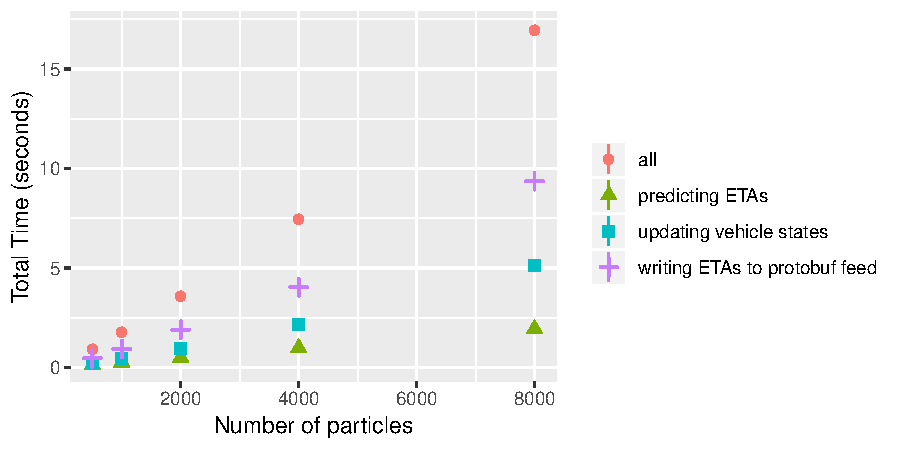
\includegraphics[width=0.7\textwidth]{figures/04_model_results_timing.pdf}
    \caption{The timings for various parts of the application, and overall. %
        The trend is slightly non-linear due to the complexity of the ETA generation step, %
        which requires sorting of the particle ETAs to obtain quantile estimates.}
    \label{fig:timings}
\end{figure}




\subsection{Model performance}
\label{sec:model_perf}


The model was evaluated using several statistics,
each calculated using a range of parameter values.
The first is effective sample size,
defined in (\ref{eq:neff}),
which is used to determined if resampling is required.
Another important statistic is the \emph{degeneration rate},
or the percent of iterations where the particle filter
is unable to find any plausible states given the observation,
and the vehicle is reinitialised.
Note, however, that some observations are \emph{invalid trips},
in which the vehicle is logged in to the wrong trip,
or ``off duty'' while still transmitting for a trip.
Some of these can be filtered for being excessively far from the route,
but others---for example traveling the wrong direction---cannot be.
The last statistic we compute is the variance of road segment travel times
over time.
For this example, we varied the number of particles $N$,
GPS error $\epsilon$, and system noise $\sigma^2$.


The one parameter we can investigate from the data is GPS error, $\epsilon^2$,
by looking at the distance between observations and the shape.
Figure~\ref{fig:dist_to_route} shows the distribution of distance between the vehicle
observation and the \emph{nearest point on the path}.
We see two peaks,
one at about 1m, and another at 2.5m.
The first of these is possibly an artefact of the data,
for example automated waypoints at intersections.
We have explored a range of GPS error values from 1 to 5~m.

\begin{figure}[tb]
    \centering
    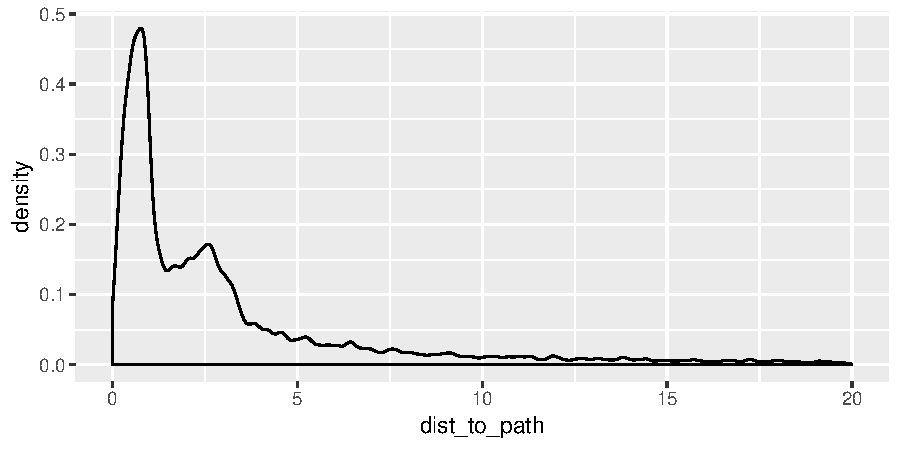
\includegraphics[width=0.7\textwidth]{figures/04_model_results_dist.pdf}
    \caption{The distance between the observation and the nearest point on the shape.}
    \label{fig:dist_to_route}
\end{figure}


For the effective sample size, 
increasing GPS error and system error both tend to
increase $N_\text{eff}$, as shown in Figure~\ref{fig:degen_rate}.
Increasing the GPS error distributes the weights more evenly,
while increasing system noise allows more particles to reach
the necessary speed,
so these are as expected.

\begin{figure}[tb]
    \centering
    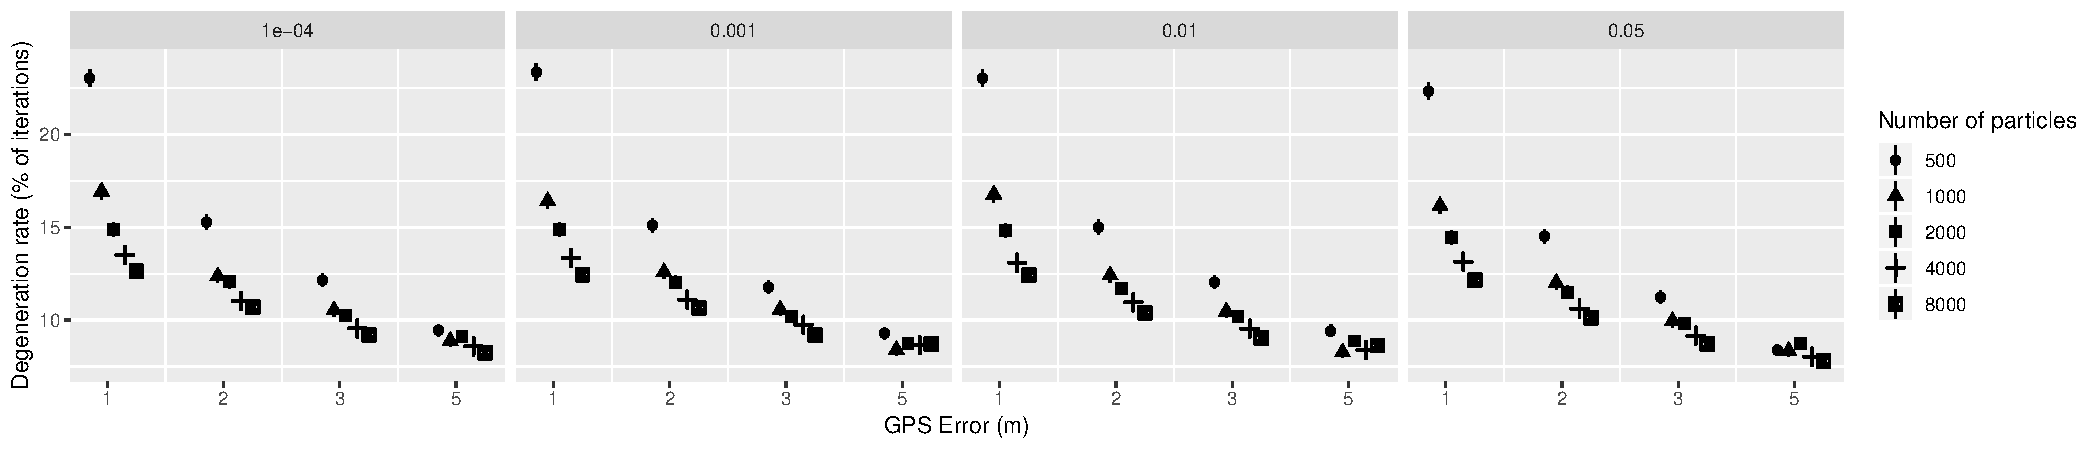
\includegraphics[width=0.9\textwidth]{figures/04_model_results_degen.pdf}
    \caption{The effective sample size and degeneration rate for a range of parameter 
        values. The columns are of increasing number of particles,
        and the rows are for increasing (downwards) GPS error.}
    \label{fig:degen_rate}
\end{figure}

The degeneration rate, 
shown on the $y$-axis of Figure~\ref{fig:degen_rate},
decreases as GPS error increases,
as anomolous observations where the bus is far from the route
are more likely.
It also decreases with the number of particles,
while system noise has no apparent effect.


Lastly is the uncertainty of travel time estimates,
as shown in Figure~\ref{fig:travel_times}.
System noise again shows no effect on the variability of travel time estimates,
however increasing GPS error tends to increase travel time variability.
This means that there is a trade-off between the models performance
and how well it estimates the main parameter of interest:
larger values of $\epsilon$ result in less degeneration and larger $N_\text{eff}$,
at the cost of more variable travel time estimates.


\begin{figure}[tb]
    \centering
    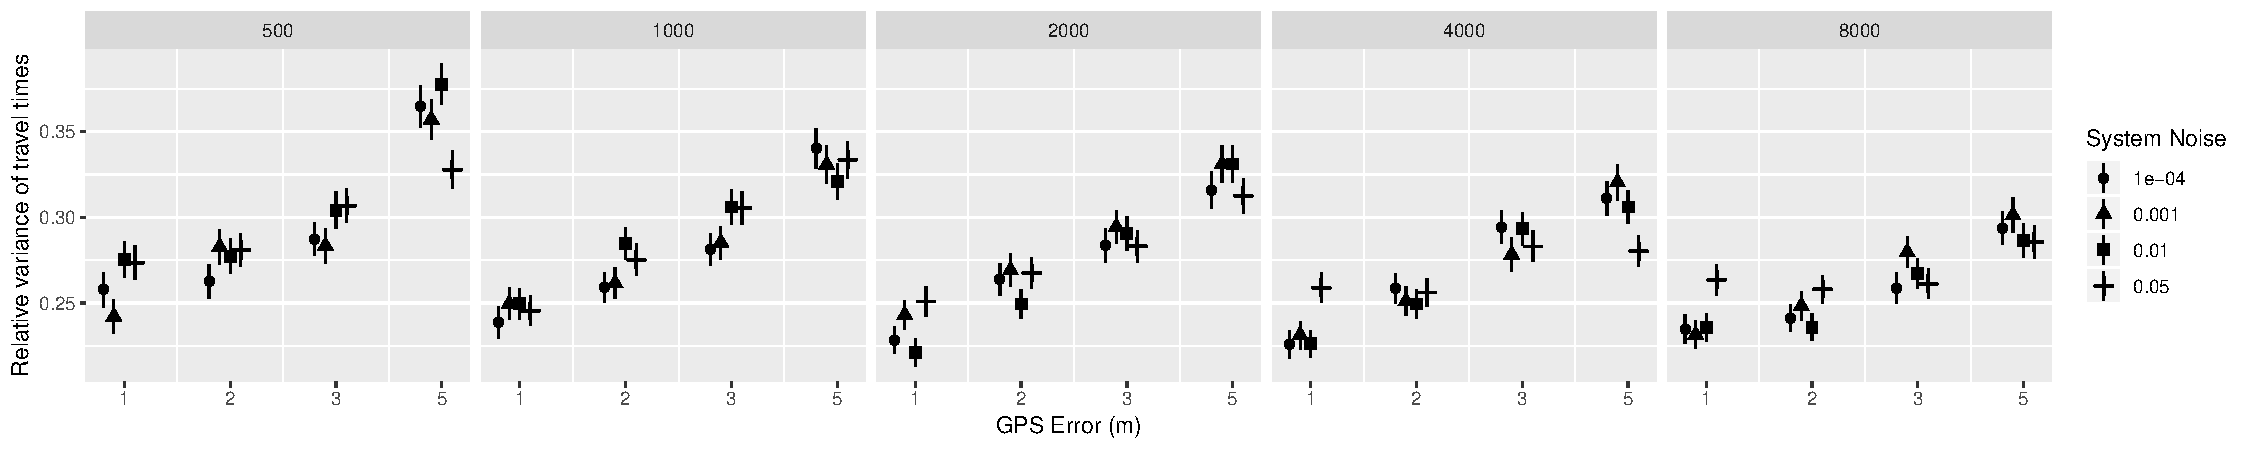
\includegraphics[width=0.9\textwidth]{figures/04_model_results_times.pdf}
    \caption{The within-segment posterior travel time uncertainty (standard error), subset by number of particles.}
    \label{fig:travel_times}
\end{figure}


